\section{Nota teórica}
\subsection*{Arduino Nano 33 Ble Sense}
El arduino Nano 33 BLE Sense es un módulo miniatura que contiene un módulo NINA B306, basado en Nordic nRF52480 y contiene un M4F Cortex, un cripto chip el cual puede almacenar certificados de forma segura y pre-compartir llaves y un IMU de 9 ejes. El módulo puede ser montado como un componente DIP o como componente SMT, directamente soldado por la vía de los pads. Es importante mencionar que la parte de TinyML forma parte de este proyecto, ya que implica reconocimiento de voz, por tanto, hay entrenamiento previo con la grabación de las acciones que se desean realizar, es decir, abrir y cerrar más dos complementos adicionales como sonidos desconocidos y ruido esto porque un modelo de ML no tiene idea sobre las cosas que están bien o mal, y solo aprende con los datos que se le dan, en ese sentido, entre más variado sean los datos, el modelo trabajará mejor \cite{web5}. Ahora, también es importante mencionar que la librería PDM y el sensor MP34DT05 ayudaron a la captura de las muestras esto porque los micrófonos se encargan de hacer la conversión de de sonidos en datos digitales.
\begin{figure}[H]
\centering
\includegraphics[width=.55\linewidth]{Img/Nano33_ble_sense_microphone.png}
 \caption{Ubicación del micrófono. Tomado de \cite{web6}.}
 \label{fig_micro}
\end{figure}


\subsubsection*{Características generales}
Las características más importantes de este mcu se mencionan a continuación \cite{web}
\begin{multicols}{2}
 \begin{itemize}
    \item CPU: ARM Cortex-M4 a 64MHz con FPU, 32-bit, 1MB Flash, 256kB SRAM.
    \item Bluetooth 5, IEEE 802.15.4-2006, \SI{2.4}{\giga\Hz}.
    \item ARM TrusZone Cryptocell 310 security subsystem, secure boot.
    \item USB 2.0, QSPI, SPI.
    \item 48 GPIOs.
    \item 12-bit, ADC con 8 canales.
    \item 64 comparadores de nivel, 15 del tipo low-power.
    \item Sensor de temperatura.
    \item $4\times4$-canales PWM.
    \item Periféricos de audio: I2S, PDM
    \item $5\times32$-bit timers.
    \item $4\times$ SPI maestros\/$3\times$ SPI esclavos.
    \item $2\times$I2C.
    \item $2\times$ UART.
    \item decodificador de cuadratura (QDEC).
    \item $3\times$ RTC.
\end{itemize}   
\end{multicols}

\subsubsection*{Diagrama de bloques}
La figura \ref{fig1} representa el diagrama de bloques de la placa.
\begin{figure}[H]
\centering
\includegraphics[width=.55\linewidth]{Img/1.png}
 \caption{Diagrama de bloques del Nano BLE 33 Sense . Tomado de \cite{web}.}
 \label{fig1} 
\end{figure}
\newpage
\subsubsection*{Diagrama de pines}
El diagrama de la figura \ref{fig2} brinda de manera más detallada la distribución de los pines.
\begin{figure}[H]
\centering
\includegraphics[width=.55\linewidth]{Img/2.png}
 \caption{Diagrama de pines del Nano BLE 33 Sense . Tomado de \cite{web2}.}
 \label{fig2}
\end{figure}

\subsubsection*{Características eléctricas}
Aquí se tomaron dos referencias para tener más claro este detalle,  primero se muestran los valores máximos del mcu nRF52480 y los de la placa respectivamente.
\begin{figure}[H]
\centering
\includegraphics[width=.55\linewidth]{Img/3.png}
 \caption{Características eléctricas de nRF52480. Tomado de \cite{web}.}
 \label{fig3}
\end{figure}

\begin{figure}[H]
\centering
\includegraphics[width=.55\linewidth]{Img/3.1.png}
 \caption{ Características eléctricas de la placa. Tomado de \cite{web2}.}
 \label{fig3.1}
\end{figure}

%%%%%%%%%%%%%%%%%%%%%%%%%%%%%%%%%%% Arduino Atmega
\subsection*{Arduino Mega 2560 Rev3}
El verdadero MCU utilizado es el elegoo MEGA 2560 R3, sin embargo comparte las mismas características que el arduino, la documentación de esta última está más depurada es por esta razón que fue la que se tomó como base.

\subsubsection{Características generales}
Las características generales de este MCU se describe a continuación \cite{ArduinoMega}:
\begin{itemize}
    \item Rendimiento de hasta 16 MIPS a 16 MHz
    \item 256k bytes (de los cuales 8k se utilizan para el cargador de arranque)
    \item 4k bytes EEPROM
    \item 8k bytes de SRAM interna
    \item 32 × 8 registros de trabajo de propósito general
    \item Contador en tiempo real con oscilador separado
    \item Cuatro canales PWM de 8 bits
    \item Cuatro USART serie programables
    \item Interfaz serie SPI controladora/periférica
\end{itemize}

\subsubsection{Diagrama de bloques}
\begin{figure}[H]
    \centering
    \includegraphics[width=.6\linewidth]{Img/k1.png}
    \caption{ Diagrama de bloques del arduino mega 2560 REV3 \cite{ArduinoMega}.}
\end{figure}

\subsubsection{Diagrama de pines}
\begin{figure}[H]
    \centering
    \includegraphics[width=.6\linewidth]{Img/k2.png}
    \caption{ Diagrama de pines del arduino mega 2560 REV3 \cite{ArduinoMega}.}
\end{figure}

\subsubsection{Características eléctricas}
\begin{figure}[H]
    \centering
    \includegraphics[width=.6\linewidth]{Img/k3.png}
    \caption{ Condiciones de operación del arduino mega 2560 REV3 \cite{ArduinoMega}.}
\end{figure}

\subsection*{Periféricos utilizados}
Los principales periféricos para este proyecto fueron el módulo I2C y el sensor MP34DT05.\par
% Escribir algo de teoría de I2C.
La idea de usar este módulo es incorporarlo con la pantalla lcd porque facilita la conexión con el arduino Mega2560 por lo que solo basta con conectar los pines \texttt{GND},\texttt{VCC},\texttt{SDA} y \texttt{SCL} de la figura \ref{fig_i2c}, donde los dos últimos tienen que ver los datos seriales y el reloj. Donde una condición de parada: alto-bajo corresponde a la transición SDA (I/O) mientras que SCL está en alto y es enviada por el \texttt{master}. Otro detalle es que estos pines necesitan resistencias de pull-up apropiadas y tomar en consideración la capacitancia total de todos los esclavos del bus I$^2$C. Los dos primeros pines se trata de una conexión básica, fuente a tierra y la alimentación del módulo que esto va conectado con los \SI{5}{\volt} del arduino Mega2560 \cite{web8}.\par
Por otro lado, el sensor MP34DT05 es un micrófono ultra-compacto que usa PDM (modulación densidad de pulso) para representar una señal analógica como una señal binaria. El rango del sensor posee diferentes valores:
\begin{itemize}
    \item Radio señal de ruido: \SI{64}{\dB}.
    \item Sensibilidad: $-26\text{dBFS} \pm \SI{3}{\dB} $
    \item Rango de temperatura: -40 a $\SI{85}{\celsius}$
\end{itemize}

\subsection*{Componentes electrónicos complementarios}
En función de cumplir con los objetivos del proyecto los siguientes componentes fueron de gran ayuda para cumplirlos.
\subsubsection*{Keypad}
La función del Keypad es para escribir la clave que se mostrará en la pantalla lcd.
\begin{figure}[H]
    \centering
    \includegraphics[width=.4\linewidth]{Img/keypad.jpg}
    \caption{Keypad}
    \label{fig_keypad}
\end{figure}
\subsubsection*{Módulo I2C}
Este componente es sumamente importante porque se incorpora a la pantalla lcd para establecer la comunicación con el microcontrolador y luego con el keypad.
\begin{figure}[H]
    \centering
    \includegraphics[width=.4\linewidth]{Img/i2c.jpg}
    \caption{Módulo I2C.}
    \label{fig_i2c}
\end{figure}
\subsubsection*{Pantalla lcd}
Su tarea es mostrar la entrada del usuario, si escribe la contraseña correcta o incorrecta se mostrará un mensaje en la pantalla.
\begin{figure}[H]
    \centering
    \includegraphics[width=.4\linewidth]{Img/lcd.jpg}
    \caption{Pantalla lcd.}
    \label{fig_lcd}
\end{figure}
\subsubsection*{Servomotor}
Este componente se encarga de abrir o cerrar la puerta dependiendo de dos aspectos. El primero es con la clave escrita en el keypad y lo segundo con base a las palabras claves: \textit{abrir} o \textit{cierra}.
\begin{figure}[H]
    \centering
    \includegraphics[width=.4\linewidth]{Img/servo.jpg}
    \caption{Servomotor.}
    \label{fig_servo}
\end{figure}
Ahora, por medio de muchas pruebas realizadas se determinó que no fue posible trabajar solo con el Arduino Nano 33 Ble Sense ya que se determinó en el laboratorio que el pin de \SI{5}{\volt} no funcionaba porque mostraba una salida de \SI{5}{\volt}. El otro problema que se mostró fue a la hora de hacer la conexión con el keypad porque a la hora de presionar cualquier botón por medio del monitor serial se estaban reconociendo caracteres completamente desconocidos, ante esto se diseñó un filtro RC en la salida, esto para las pulsaciones, sin embargo, el problema persistía. El otro problema es con la pantalla lcd, ella necesita una alimentación de al menos \SI{5}{\volt}, en ese sentido debe estar conectada a un pin que posee esa salida, de lo contrario muestra un bajo contraste y no se puede apreciar correctamente el contenido, para solucionar este problema pudo haberse hecho un par Darlington o realizar lo mostrado en la figura \ref{fig_usb}.

\begin{figure}[H]
    \centering
    \includegraphics[width=.4\linewidth]{Img/pin_vusb.png}
    \caption{Habilitación de \SI{5}{\volt}.}
    \label{fig_usb}
\end{figure}
No obstante, por cuestiones de tiempo y complejidad en ese tipo de soldadura especial/fina no se tomaron esos caminos. Ante todos estas situaciones lo más favorable fue hacer uso de otra placa para realizar estas conexiones. Entonces, el proyecto tiene dos etapas:
\begin{itemize}
    \item La placa Arduino MEGA2560, se encarga de abrir y cerrar la puerta por medio del keypad cuando se le escribe la contraseña correcta y controlar el display.
    \item La placa Arduino Nano 33 Ble Sense fue entrenada con 4 clases; dos keywords (abrir/cerrar) y otras dos con ruido y sonidos desconocidos. Así, cuando reconozca alguna de las palabras claves se abrirá o cerrará la puerta y encenderá un LED dependiendo del estado.
\end{itemize}

% TABLA DE COMPONENTES
\begin{table}[H]
\caption{Lista de equipos}
\label{table_2}
\begin{center}
\begin{tabular}{r|cc}
\hline
\textbf{Componente}&\textbf{Cantidad}&\textbf{Precio}\\
 \hline
Arduino Nano 33 Ble Sense& 1 &60\$ \\ \hline 
Arduino Mega2560& 1 & 18\$ \\ \hline 
Keypad& 1 &9\$ \\ \hline 
Pantalla lcd& 1 &6.95\$ \\ \hline 
Servomotor& 2 &11\$ \\ \hline 
Batería \SI{9}{\volt}& 1 &5.5\$ \\ \hline 
Kit de resistencias& 1 & 0.2\$ \\ \hline 
Kit de jumpers & 1 &2 \$ \\ \hline 
Módulo I2C & 1 & 4\$ \\ \hline 

 \textbf{Total}& & 117\$ \\
 \hline
\end{tabular}
\end{center}
\end{table}

\subsection*{Diseño del circuito}
\begin{figure}[H]
    \centering
\tikzset{every picture/.style={line width=0.75pt}} %set default line width to 0.75pt        

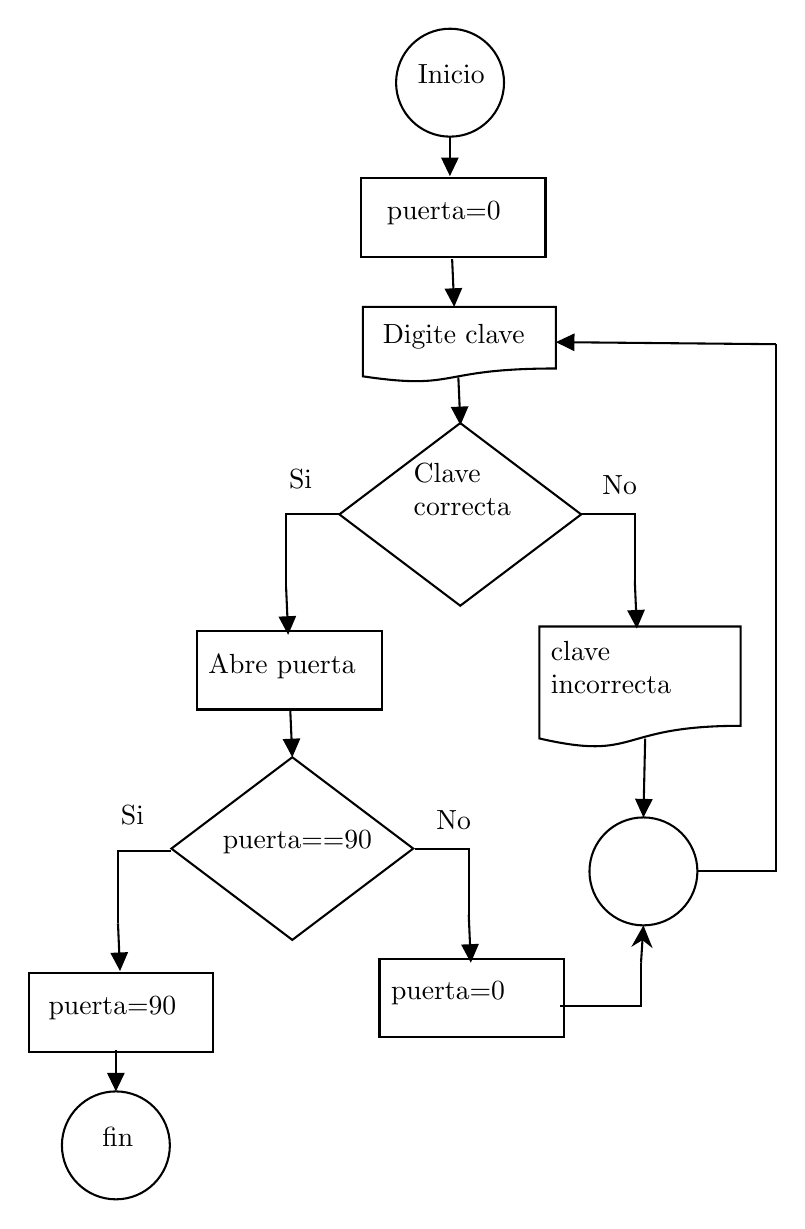
\begin{tikzpicture}[x=0.75pt,y=0.75pt,yscale=-1,xscale=1]
%uncomment if require: \path (0,649); %set diagram left start at 0, and has height of 649

%Flowchart: Connector [id:dp42585090626324207] 
\draw   (304,59) .. controls (304,44.64) and (315.64,33) .. (330,33) .. controls (344.36,33) and (356,44.64) .. (356,59) .. controls (356,73.36) and (344.36,85) .. (330,85) .. controls (315.64,85) and (304,73.36) .. (304,59) -- cycle ;
%Straight Lines [id:da9927818650372262] 
\draw    (329.92,85) -- (329.92,101) ;
\draw [shift={(329.92,104)}, rotate = 270] [fill={rgb, 255:red, 0; green, 0; blue, 0 }  ][line width=0.08]  [draw opacity=0] (8.93,-4.29) -- (0,0) -- (8.93,4.29) -- cycle    ;
%Flowchart: Decision [id:dp8222109791046812] 
\draw   (334.92,223) -- (393.17,267) -- (334.92,311) -- (276.67,267) -- cycle ;
%Shape: Right Angle [id:dp5468713947182464] 
\draw   (276.67,267) -- (251,267) -- (251,302) ;
%Straight Lines [id:da34123972616362797] 
\draw    (251,302) -- (251.87,322) ;
\draw [shift={(252,325)}, rotate = 267.51] [fill={rgb, 255:red, 0; green, 0; blue, 0 }  ][line width=0.08]  [draw opacity=0] (8.93,-4.29) -- (0,0) -- (8.93,4.29) -- cycle    ;
%Flowchart: Process [id:dp6422094052668206] 
\draw   (208,323) -- (297,323) -- (297,361) -- (208,361) -- cycle ;
%Shape: Right Angle [id:dp9632380337734168] 
\draw   (393.17,267) -- (419,267) -- (419,299) ;
%Straight Lines [id:da9224648988654192] 
\draw    (419,299) -- (419.87,319) ;
\draw [shift={(420,322)}, rotate = 267.51] [fill={rgb, 255:red, 0; green, 0; blue, 0 }  ][line width=0.08]  [draw opacity=0] (8.93,-4.29) -- (0,0) -- (8.93,4.29) -- cycle    ;
%Straight Lines [id:da14093121348085114] 
\draw    (424,375) -- (423.23,410) ;
\draw [shift={(423.17,413)}, rotate = 271.26] [fill={rgb, 255:red, 0; green, 0; blue, 0 }  ][line width=0.08]  [draw opacity=0] (8.93,-4.29) -- (0,0) -- (8.93,4.29) -- cycle    ;
%Flowchart: Connector [id:dp28231580529895073] 
\draw   (143,571) .. controls (143,556.64) and (154.64,545) .. (169,545) .. controls (183.36,545) and (195,556.64) .. (195,571) .. controls (195,585.36) and (183.36,597) .. (169,597) .. controls (154.64,597) and (143,585.36) .. (143,571) -- cycle ;
%Flowchart: Document [id:dp7887811718871025] 
\draw   (373,321) -- (470,321) -- (470,368.85) .. controls (409.38,368.85) and (421.5,386.1) .. (373,374.94) -- cycle ;
%Shape: Right Angle [id:dp7465732461480319] 
\draw   (449.17,439) -- (487,439) -- (487,185) ;
%Straight Lines [id:da9427213356074324] 
\draw    (384,184.03) -- (487,185) ;
\draw [shift={(381,184)}, rotate = 0.54] [fill={rgb, 255:red, 0; green, 0; blue, 0 }  ][line width=0.08]  [draw opacity=0] (8.93,-4.29) -- (0,0) -- (8.93,4.29) -- cycle    ;
%Flowchart: Connector [id:dp6793358076053446] 
\draw   (397.17,439) .. controls (397.17,424.64) and (408.81,413) .. (423.17,413) .. controls (437.53,413) and (449.17,424.64) .. (449.17,439) .. controls (449.17,453.36) and (437.53,465) .. (423.17,465) .. controls (408.81,465) and (397.17,453.36) .. (397.17,439) -- cycle ;
%Straight Lines [id:da6157101498528812] 
\draw    (253,361) -- (253.87,381) ;
\draw [shift={(254,384)}, rotate = 267.51] [fill={rgb, 255:red, 0; green, 0; blue, 0 }  ][line width=0.08]  [draw opacity=0] (8.93,-4.29) -- (0,0) -- (8.93,4.29) -- cycle    ;
%Flowchart: Process [id:dp10984865947746725] 
\draw   (296,481) -- (385,481) -- (385,519) -- (296,519) -- cycle ;
%Flowchart: Process [id:dp2789359345260862] 
\draw   (287,105) -- (376,105) -- (376,143) -- (287,143) -- cycle ;
%Straight Lines [id:da14083283346218511] 
\draw    (334,201) -- (334.87,221) ;
\draw [shift={(335,224)}, rotate = 267.51] [fill={rgb, 255:red, 0; green, 0; blue, 0 }  ][line width=0.08]  [draw opacity=0] (8.93,-4.29) -- (0,0) -- (8.93,4.29) -- cycle    ;
%Flowchart: Decision [id:dp06088544865395984] 
\draw   (254,384) -- (312.25,428) -- (254,472) -- (195.75,428) -- cycle ;
%Shape: Right Angle [id:dp8217099184396621] 
\draw   (313.17,428) -- (339,428) -- (339,460) ;
%Straight Lines [id:da965375327404175] 
\draw    (339,460) -- (339.87,480) ;
\draw [shift={(340,483)}, rotate = 267.51] [fill={rgb, 255:red, 0; green, 0; blue, 0 }  ][line width=0.08]  [draw opacity=0] (8.93,-4.29) -- (0,0) -- (8.93,4.29) -- cycle    ;
%Shape: Right Angle [id:dp7886934725142394] 
\draw   (195.67,429) -- (170,429) -- (170,464) ;
%Straight Lines [id:da8518021831322284] 
\draw    (170,464) -- (170.87,484) ;
\draw [shift={(171,487)}, rotate = 267.51] [fill={rgb, 255:red, 0; green, 0; blue, 0 }  ][line width=0.08]  [draw opacity=0] (8.93,-4.29) -- (0,0) -- (8.93,4.29) -- cycle    ;
%Flowchart: Process [id:dp8640224184714345] 
\draw   (127,488) -- (216,488) -- (216,526) -- (127,526) -- cycle ;
%Shape: Right Angle [id:dp5762038720241354] 
\draw   (383,504) -- (422,504) -- (422,483) ;
%Straight Lines [id:da6437862550472608] 
\draw    (422,483) -- (422.97,467.99) ;
\draw [shift={(423.17,465)}, rotate = 93.71] [fill={rgb, 255:red, 0; green, 0; blue, 0 }  ][line width=0.08]  [draw opacity=0] (10.72,-5.15) -- (0,0) -- (10.72,5.15) -- (7.12,0) -- cycle    ;
%Flowchart: Document [id:dp3979180887556457] 
\draw   (288,167) -- (381,167) -- (381,196.7) .. controls (322.88,196.7) and (334.5,207.41) .. (288,200.48) -- cycle ;
%Straight Lines [id:da5018025676967481] 
\draw    (331,144) -- (331.87,164) ;
\draw [shift={(332,167)}, rotate = 267.51] [fill={rgb, 255:red, 0; green, 0; blue, 0 }  ][line width=0.08]  [draw opacity=0] (8.93,-4.29) -- (0,0) -- (8.93,4.29) -- cycle    ;
%Straight Lines [id:da6767101156206579] 
\draw    (169,525) -- (169,542) ;
\draw [shift={(169,545)}, rotate = 270] [fill={rgb, 255:red, 0; green, 0; blue, 0 }  ][line width=0.08]  [draw opacity=0] (8.93,-4.29) -- (0,0) -- (8.93,4.29) -- cycle    ;

% Text Node
\draw (313,49) node [anchor=north west][inner sep=0.75pt]   [align=left] {Inicio};
% Text Node
\draw (250.92,244) node [anchor=north west][inner sep=0.75pt]   [align=left] {Si};
% Text Node
\draw (212.08,332.67) node [anchor=north west][inner sep=0.75pt]   [align=left] {Abre puerta};
% Text Node
\draw (311,241) node [anchor=north west][inner sep=0.75pt]   [align=left] {Clave\\correcta\\};
% Text Node
\draw (401.92,247) node [anchor=north west][inner sep=0.75pt]   [align=left] {No};
% Text Node
\draw (161,561) node [anchor=north west][inner sep=0.75pt]   [align=left] {fin};
% Text Node
\draw (377.08,326.67) node [anchor=north west][inner sep=0.75pt]   [align=left] {clave\\incorrecta};
% Text Node
\draw (300.08,490.67) node [anchor=north west][inner sep=0.75pt]   [align=left] {puerta=0};
% Text Node
\draw (298.08,114.67) node [anchor=north west][inner sep=0.75pt]   [align=left] { puerta=0};
% Text Node
\draw (219,418) node [anchor=north west][inner sep=0.75pt]   [align=left] {puerta==90};
% Text Node
\draw (321.92,408) node [anchor=north west][inner sep=0.75pt]   [align=left] {No};
% Text Node
\draw (169.92,406) node [anchor=north west][inner sep=0.75pt]   [align=left] {Si};
% Text Node
\draw (135.08,497.67) node [anchor=north west][inner sep=0.75pt]   [align=left] {puerta=90};
% Text Node
\draw (296.08,173.67) node [anchor=north west][inner sep=0.75pt]   [align=left] {Digite clave};


\end{tikzpicture}

    \caption{Diagrama de bloques smart door lock.}
    \label{sch_1}
\end{figure}
El diagrama mostrado anteriormente es la lógica que posee el proyecto en general. Gracias a este esquema, desde un inicio se tuvo claro los objetivos a cumplir.
%\newpage
